\documentclass[__main__.tex]{subfiles}

\begin{document}

\section{Метод матричной прогонки для численного решения двумерного параболического уравнения в частных производных с неявной разностной схемой}

Рассмотрим задачу Коши:

\begin{equation} \label{50.1}
\begin{cases}
\frac{\partial U}{\partial t} = \frac{\partial^2 U}{\partial x^2} + \frac{\partial^2 U}{\partial y^2}, (t, x, y) \in [0, T] x (a, b)^2 \\
U(0,x,y) = \mu(x,y), \ (x,y)\in [a;b]^2 \\
U(t,a,y) = \alpha(t,y), \ (t,y)\in [0, T] x [a;b] \\
U(t,b,y) = \beta(t,y), \\
U(t,x,a) = \gamma(t,x), \\
U(t,x,b) = \psi(t,x), \\
\end{cases}
\end{equation}

Для численного решения задачи (1) на квадрате $[a,b]^2$ рассмотрим двумерную равномерную сетку:

\begin{equation}\label{50.2}
<(x_k, y_m): k = \overline{0,K+1}, n = \overline{0,M+1}>
\end{equation}

где $x_k-x_{k-1} = h$ для $k = \overline{1,K+1}$ и $y_m-x_{m-1} = h$ для $m = \overline{1,M+1}$
$$
(x_0 = a, x_{k+1} = b, y_0 = a, y_{m+1} = b)
$$

Для отрезка $[0, T]$ введем равномерную сетку 

\begin{equation}\label{50.3}
<0=t^0, t^1 .. t^N = T>, t^n - t^{n-1} = \tau, n = \overline{0,N}
\end{equation}

Если $h, \tau \rightarrow 0$ и рассм-ся при фикс. $h, \tau$ разностный аналог задачи (1) для неявной схемы, индуцированный шаблоном:

\begin{figure}[ht]
	\centering
	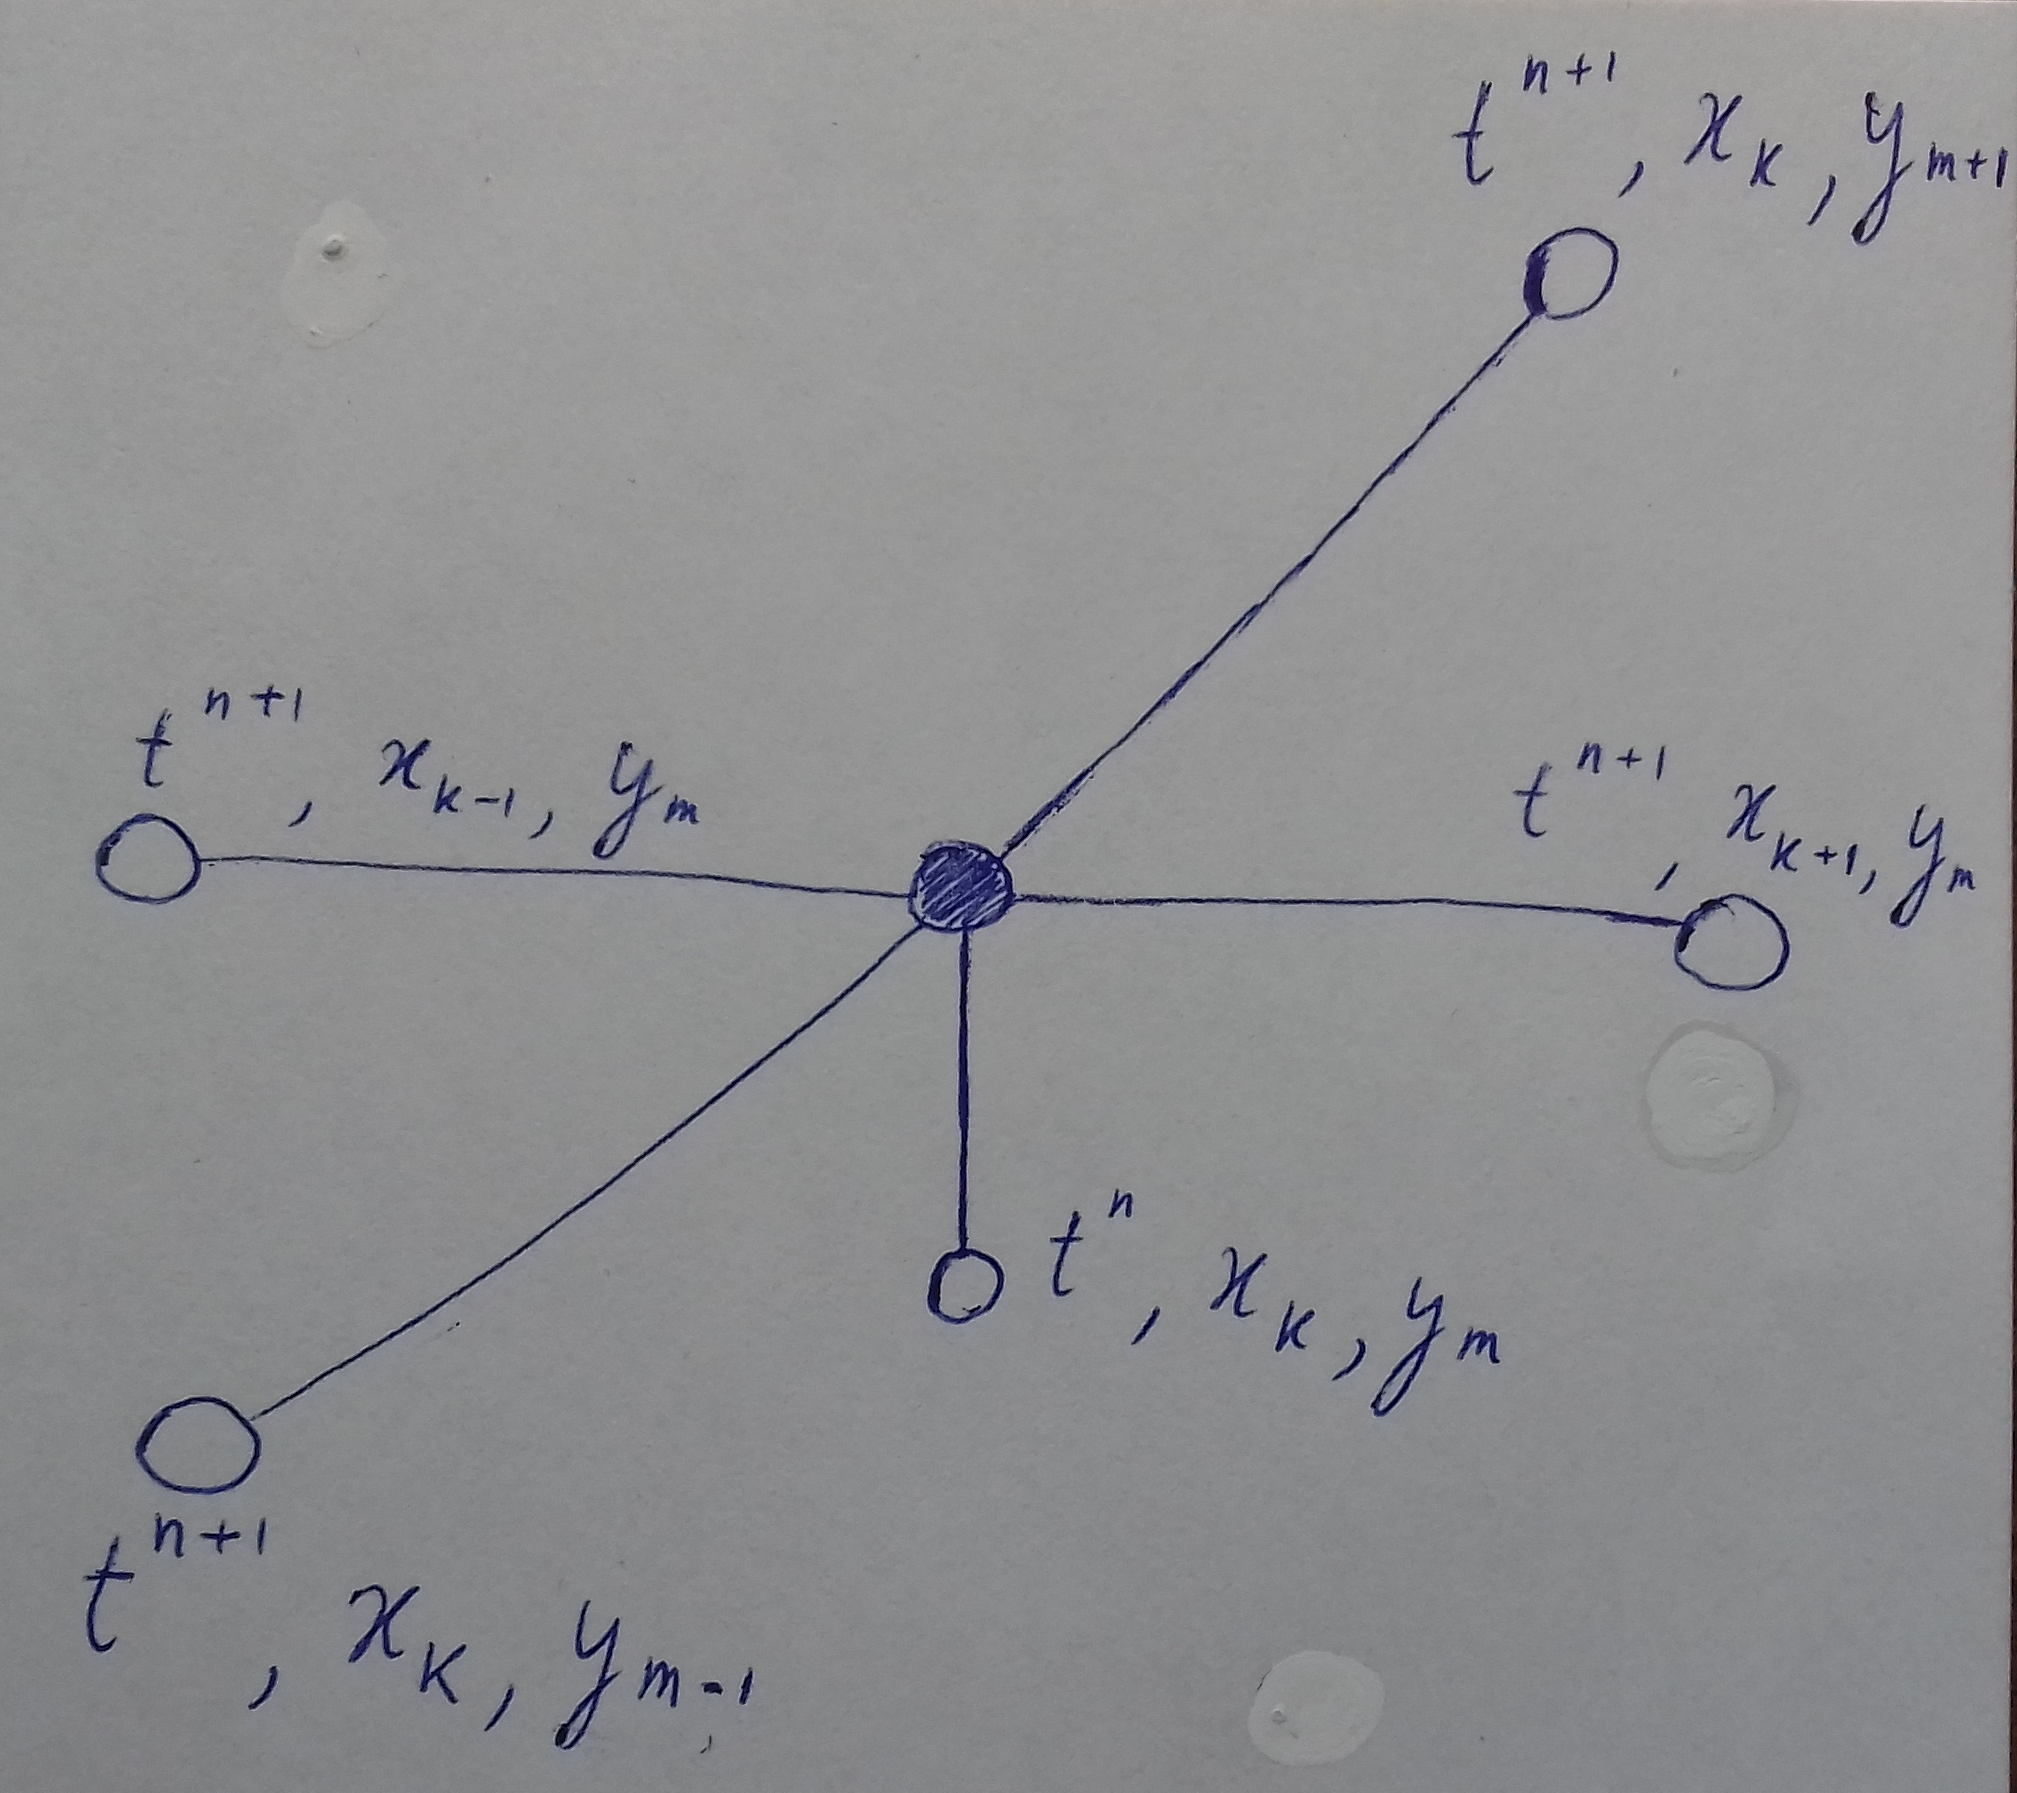
\includegraphics[width=0.4\linewidth]{img/img_50_1}
	\caption{}
	\label{img_42.1}
\end{figure}

Схема будет аппроксимировать задачу (1) с порядком аппроксимации $ \tau, h^2 $.

\begin{equation} \label{50.4}
\begin{cases}
$$\frac{U^{n+1}_{k,m} - U^{n}_{k,m}}{\tau}$$ = $$\frac{U^{n+1}_{k-1,m} - 2U^{n+1}_{k,m} + U^{n+1}_{k+1,m}}{h^2}$$ + $$\frac{U^{n+1}_{k,m-1} - 2U^{n+1}_{k,m} + U^{n+1}_{k,m+1}}{h^2}$$ \\
n = \overline{0,N-1}, \ k = \overline{1,K}, \ m = \overline{1,M} \\
U^0_{k,m} = \mu_{k,m}, \\ 
U^n_{0,m} = \alpha^n_{m}, \ U^n_{k+1,m} = \beta^n_{m}, \\
U^n_{k,0} = \gamma^n_{k}, \ U^n_{k,m+1} = \psi^n_{k}
\end{cases}
\end{equation}

Согласно аналогу (4) введем обозначение: $\;^{>}U^n_k = \left(
\begin{matrix}
U^n_{k,1}  \\
U^n_{k,2}   \\
...  \\
U^n_{k,m}  
\end{matrix}
\right)$ и $n = \overline{0,N}, k = \overline{0,K+1}$

Используя это обозначение и $\text{\ae} = \tau/h^2$ из (4) получим:

\begin{equation}\label{50.5}
-\text{\ae} \cdot U^{n+1}_{k,m-1} - \text{\ae} \cdot U^{n+1}_{k-1,m} + (1 - 4\text{\ae}) \cdot U^{n+1}_{k,m} - \text{\ae} \cdot U^{n+1}_{k+1,m} - \text{\ae} \cdot U^{n+1}_{k,m+1} = U^{n}_{k,m}
\end{equation}

\begin{equation}\label{50.6}
-A \cdot U^{n+1}_{k-1} + B \cdot U^{n+1}_{k} - C \cdot U^{n+1}_{k+1} = \;^{>}d_k
\end{equation}

$d_k = \left(
\begin{matrix}
U^n_{k,1} + \text{\ae} \cdot \gamma^n_{k} \\
U^n_{k,2}   \\
...  \\
U^n_{k,m-1} \\
U^n_{k,m} + \psi^n_{k} 
\end{matrix}
\right)$

A = $C = \left(
\begin{matrix}
\text{\ae} & ... & 0 \\
0 &... & \text{\ae}
\end{matrix}
\right)$ = $\text{\ae} \cdot E_m$

B = $G_k = \left(
\begin{matrix}
1 + 4 \cdot \text{\ae} & -\text{\ae} & ... & ... & ... & ... \\
-\text{\ae} & 1 + 4 \cdot \text{\ae} & -\text{\ae} & ... &... & ... \\
... & ... & ... & ... & ... & ... \\
0 & ... & ... & -\text{\ae} & 1 + 4\text{\ae} & -\text{\ae} \\
0 & ... & ... & ... & -\text{\ae} & 1 + 4\text{\ae}
\end{matrix}
\right)$

Для реш-я СЛАУ (6) исп-ем матричную прогонку, т.е. полагаем для $\forall k = \overline{1,K}$ формулу:

\begin{equation}\label{50.7}
\;^{>}U_k = L_{k+1} \cdot \;^{>}U^{n+1}_{k+1} + \;^{>}M_{k+1}, k = \overline{0,K}
\end{equation}

Поскольку $\;^{>}U^{n+1}_0 = \;^{>}\alpha^{n+1} = \left(
\begin{matrix}
\;^{>}\alpha^{n+1}_{0,1} \\
...  \\
\;^{>}\alpha^{n+1}_{0,m}
\end{matrix}
\right)$, то в (7):

\begin{equation}\label{50.8}
L_1 = \left(
\begin{matrix}
0 & ... & 0 \\
0 & ... & 0
\end{matrix}
\right)
\end{equation}

причем $\;^{>}M_{k+1} = \;^{>}\alpha^{n+1}$. Тогда получаем:

$$
-A \cdot U^{n+1}_{0} + B \cdot U^{n+1}_{1} - C \cdot U^{n+1}_{2} = \;^{>}d_1 \Rightarrow 
\Rightarrow B \cdot U^{n+1}_{1} = C \cdot U^{n+1}_{2} + (\;^{>}d_1 + A \cdot U^{n+1}_{0}) \Rightarrow
\Rightarrow U^{n+1}_{1} = B^{-1} \cdot C \cdot U^{n+1}_{2} + B^{-1} \cdot (\;^{>}d_1 + A \cdot U^{n+1}_{0}) \Rightarrow L_2 + U^{n+1}_{2} + M^2_2
$$

где $L_2 = B^{-1} \cdot C$, $\;^{>}M_2 = B^{-1} \cdot (\;^{>}d_1 + A \cdot \;^{>}U^{n+1}_0)$

Аналогично:

$\;^{>}U^{n+1}_2 = L_{k+3} \cdot \;^{>}U^{n+1}_{3} + \;^{>}M_{k+1}, k = \overline{0,K},$

где, согласно (6):

$$
- A \cdot U^{n+1}_{1} + B \cdot U^{n+1}_{2} - C \cdot U^{n+1}_{3} = \;^{>}d^n_2 \Rightarrow 
\Rightarrow - A \cdot (L_{2} \cdot \;^{>}U^{n+1}_{2} + \;^{>}M_{2}) + B \cdot U^{n+1}_{2} = C \cdot \;^{>}U^{n+1}_{3} + \;^{>}d^n_2 + A \cdot \;^{>}M_{2}
$$

$$
U^{n+1}_{2} = (B - AL_2)^{-1}\cdot C \cdot U^{n+1}_{3} + (B - AL_2)^{-1} \cdot (\;^{>}d^n_2 + A \cdot \;^{>}M_{2})
$$

Таким образом:

$$
U^{n+1}_{k} = (B - AL_k)^{-1}\cdot C \cdot U^{n+1}_{k+1} + (B - AL_2)^{-1} \cdot (\;^{>}d^n_k + A \cdot \;^{>}M_{k})
$$

где $\;^{>}U^{n+1}_{k+1} = \;^{>}\beta^{n+1} = \left(
\begin{matrix}
\beta^{n+1}_{k+1,1} \\
...  \\
\beta^{n+1}_{k+1,m} 
\end{matrix}
\right)$, т.е. найдено $U^{n+1}_{k}$ и далее $\;^{>}U^{n+1}_{k-1} = L_{k} \cdot \;^{>}U^{n}_{k} + \;^{>}M_{k} ... U^{n+1}_1$
 
\end{document}
